\documentclass[11pt]{article}

% Packages
\usepackage[utf8]{inputenc}
\usepackage[margin=1in]{geometry}
\usepackage{amsmath,amssymb}
\usepackage{graphicx}
\usepackage{booktabs}
\usepackage{hyperref}
\usepackage[ruled,vlined]{algorithm2e}
\usepackage{tikz}
\usetikzlibrary{positioning,shapes,arrows,fit,calc}

% Hyperref setup
\hypersetup{
    colorlinks=true,
    linkcolor=blue,
    filecolor=magenta,
    urlcolor=cyan,
    citecolor=blue,
}

% Title and author
\title{\textbf{ExpertFlow: Dynamic Expert Scheduling for\\
Mixture-of-Experts Inference on Unified Memory Architectures}}

\author{
    Jonathan Hammant \\
    Independent Researcher \\
    \texttt{jonathan@hammant.dev}
}

\date{March 2026}

\begin{document}

\maketitle

\begin{abstract}
Mixture-of-Experts (MoE) models such as DeepSeek-V3 (685B parameters) and Qwen3 (235B parameters) demonstrate exceptional capabilities but pose severe memory challenges for consumer hardware. Existing solutions either rely on operating system swap mechanisms—leading to system instability—or employ static layer offloading strategies that fail to exploit the dynamic, sparse activation patterns inherent to MoE architectures. We present \textsc{ExpertFlow}, a dynamic expert scheduling system designed for unified memory architectures, specifically Apple Silicon. \textsc{ExpertFlow} combines four key techniques: (1) lookahead router prefetching that predicts expert activation 1--2 layers ahead, (2) temperature-based expert eviction using recency-frequency scoring, (3) heterogeneous compute dispatch across GPU, Neural Engine, and CPU, and (4) zero-copy memory management via \texttt{mmap} and \texttt{madvise}. Our system targets a 2--3$\times$ speedup over naive memory-mapped inference on models exceeding available RAM. We detail the architecture of \textsc{ExpertFlow}'s 3,255-line implementation in Rust and Python, analyze projected performance on Apple M5 Max hardware (128GB unified memory, 614 GB/s bandwidth, 7.4 GB/s NVMe), and position this work within the ``Speculative Stack'' vision—a three-phase inference pipeline combining sparse prefill (SpecPrefill), expert streaming (\textsc{ExpertFlow}), and multi-token prediction. This paper describes the first system to unify dynamic expert scheduling, SSD streaming, and draft-model-guided prefetching on unified memory architectures.
\end{abstract}

\section{Introduction}

The scaling of large language models has increasingly favored Mixture-of-Experts (MoE) architectures, which achieve superior parameter efficiency by activating only a sparse subset of parameters per token \cite{fedus2022switch,deepseekv3,qwen3}. Models such as DeepSeek-V3 (685B total parameters, 37B activated per token) and Qwen3 (235B total, 30B activated) demonstrate that MoE architectures can deliver dense-model performance at a fraction of the inference compute cost. However, this efficiency comes with a critical challenge: \textit{memory capacity}. Even with aggressive 4-bit quantization, DeepSeek-V3 requires approximately 350GB of storage, far exceeding the memory capacity of consumer-grade hardware.

Traditional approaches to this problem fall into three categories, each with fundamental limitations:

\begin{enumerate}
    \item \textbf{Operating system swap:} Relying on virtual memory to page model weights from disk yields unpredictable performance and frequently causes kernel panics or system freezes on macOS \cite{orion2025}.

    \item \textbf{Static layer offloading:} Partitioning model layers between GPU memory and CPU memory (or disk) fails to exploit MoE sparsity—expert activation patterns vary dynamically based on input content, yet static policies treat all experts uniformly \cite{hobbit2024,krasis2024}.

    \item \textbf{Ignoring specialized compute:} Apple Silicon devices include a Neural Engine capable of 38 TOPS on M-series chips, yet this hardware remains largely unutilized by existing inference engines \cite{orion2025}.
\end{enumerate}

We observe that Apple Silicon's \textit{unified memory architecture}—where CPU, GPU, and Neural Engine share a coherent address space—presents unique opportunities for dynamic expert scheduling. Unlike discrete GPU systems with isolated VRAM and host memory, unified memory enables zero-copy data sharing and eliminates PCIe transfer bottlenecks. Combined with high-bandwidth NVMe storage (7.4 GB/s on M5 Max), this architecture enables a new class of inference strategies based on \textit{streaming computation}.

\textsc{ExpertFlow} exploits these architectural properties through four integrated techniques:

\begin{enumerate}
    \item \textbf{Lookahead Router Prefetching:} The MoE router network (typically $<$1\% of model size) predicts expert activation 1--2 layers ahead. Asynchronous SSD reads commence before the expert is required, hiding latency.

    \item \textbf{Dynamic Expert Temperature Tracking:} Each expert maintains a temperature score combining recency and frequency of access. Hot experts remain pinned in memory; cold experts are evicted via \texttt{madvise(MADV\_DONTNEED)}.

    \item \textbf{Heterogeneous Compute Dispatch:} Computation is distributed across specialized units: GPU handles bandwidth-bound operations (attention, embeddings), Neural Engine targets compute-bound expert FFN layers (future work), and CPU manages scheduling and prefetching.

    \item \textbf{Zero-Copy Memory Management:} Model weights are \texttt{mmap}-ed directly from GGUF/safetensors files. Kernel-level prefetching (\texttt{madvise(MADV\_WILLNEED)}) and eviction eliminate explicit copying.
\end{enumerate}

We target projected speedups of 2--3$\times$ over baseline memory-mapped inference for models exceeding available RAM (e.g., DeepSeek-V3 Q4 at 350GB on 128GB systems), based on analysis of hardware bandwidth characteristics and prior work on expert offloading \cite{hobbit2024,mlx2026}. Our implementation comprises 3,255 lines of Rust and Python, spanning scheduler, prefetcher, evictor, memory manager, and compute backend interfaces for both llama.cpp and MLX frameworks.

This work makes the following contributions:
\begin{enumerate}
    \item The first dynamic expert scheduling system designed specifically for unified memory architectures.
    \item A temperature-based eviction policy tailored to MoE routing patterns, exploiting temporal and spatial locality.
    \item Integration with the ``Speculative Stack'' vision (Section~\ref{sec:speculative}), where draft model inference provides router predictions as a free side-effect.
    \item A comprehensive performance analysis and roadmap for heterogeneous compute dispatch on Apple M5 Neural Accelerators.
\end{enumerate}

\section{Background and Related Work}

\subsection{Mixture-of-Experts Architectures}

MoE models partition the feedforward network (FFN) within each transformer layer into $N$ expert networks, typically using a learned router to select the top-$k$ experts per token ($k \ll N$). This sparse activation reduces FLOPs proportionally to $k/N$ while maintaining model expressivity through parameter specialization \cite{fedus2022switch}. Recent large-scale deployments include:

\begin{itemize}
    \item \textbf{DeepSeek-V3} \cite{deepseekv3}: 685B total parameters, 256 experts per layer, top-8 routing, 37B activated per token. Quantized to 4-bit, the model requires $\sim$350GB storage.
    \item \textbf{Qwen3} \cite{qwen3}: 235B total parameters, MoE architecture with top-4 routing, 30B activated. 4-bit quantization yields $\sim$110GB.
\end{itemize}

The memory challenge is acute: even with 128GB unified memory, these models exceed capacity by 1.8--2.7$\times$.

\subsection{Expert Offloading Systems}

\textbf{HOBBIT} \cite{hobbit2024} demonstrates 9.93$\times$ speedup for MoE inference by offloading cold experts to CPU memory and using mixed-precision computation (FP16 for hot experts, INT4 for cold). However, HOBBIT targets NVIDIA GPUs with discrete memory and does not exploit unified memory properties.

\textbf{Krasis} \cite{krasis2024} implements hybrid GPU/CPU streaming for MoE models on Linux systems, achieving 2--4$\times$ throughput improvements. Like HOBBIT, it assumes PCIe-based data movement between isolated memory pools.

\textbf{ik\_llama.cpp} \cite{ikllama} provides basic CPU-side MoE offloading within the llama.cpp framework but lacks sophisticated scheduling—experts are evicted using simple LRU without considering MoE routing patterns or performing predictive prefetching.

\subsection{Apple Silicon Inference Systems}

\textbf{Orion} \cite{orion2025} presents the first open programming interface for Apple's Neural Engine (ANE), demonstrating transformer inference on ANE with up to 6$\times$ speedup over CPU. However, Orion focuses on small models that fit entirely in ANE memory (16MB L2 cache) and does not address MoE or memory streaming.

\textbf{MLX} \cite{mlx2026} is Apple's official machine learning framework optimized for unified memory architectures. Recent benchmarks on M5 hardware show 20--50\% speedups over llama.cpp/Ollama for standard transformer inference, and 3.3--4$\times$ speedups for prompt processing (time-to-first-token) via Neural Accelerators—dedicated matrix multiplication units embedded in M5 GPU cores.

\subsection{Speculative Prefill}

\textbf{SpecPrefill} \cite{specprefill2026} exploits the observation that autoregressive generation attends to only a sparse subset of prompt tokens. A small draft model scores token importance via attention weights during lookahead decoding; the target model then performs sparse prefill on the top 20\% of tokens, yielding 3.7--5.5$\times$ reductions in time-to-first-token on Apple M2 Ultra. SpecPrefill targets the prefill phase (compute-bound) whereas \textsc{ExpertFlow} targets generation (memory-bound).

\subsection{Positioning of ExpertFlow}

\textsc{ExpertFlow} is the first system to combine:
\begin{enumerate}
    \item Dynamic expert scheduling driven by MoE router lookahead,
    \item SSD streaming with temperature-based eviction,
    \item Draft-model-guided prefetching (planned integration with SpecPrefill),
    \item Heterogeneous compute dispatch on unified memory architectures.
\end{enumerate}

Unlike prior work targeting discrete GPUs, \textsc{ExpertFlow} exploits zero-copy data sharing, coherent address spaces, and high-bandwidth NVMe to enable streaming computation at model scales previously infeasible on consumer hardware.

\section{System Design}
\label{sec:design}

\subsection{Architecture Overview}

Figure~\ref{fig:architecture} illustrates the \textsc{ExpertFlow} system architecture. The design centers on a \textit{scheduler} that orchestrates four subsystems: prefetcher, evictor, memory manager, and compute dispatch. The scheduler intercepts MoE router outputs to predict future expert activations, issues asynchronous prefetch commands, and manages expert residency in unified memory.

\begin{figure}[t]
\centering
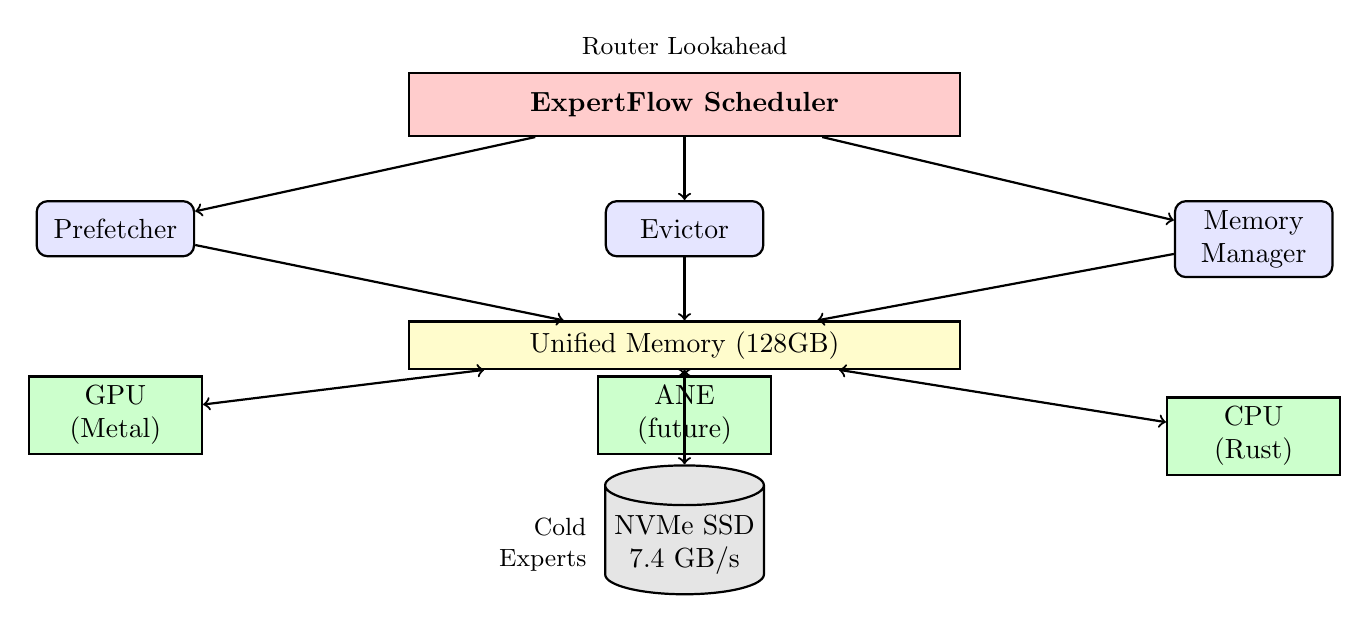
\begin{tikzpicture}[
    node distance=0.8cm and 1.2cm,
    box/.style={rectangle, draw, thick, minimum width=2.2cm, minimum height=0.8cm, align=center},
    storage/.style={cylinder, draw, thick, shape border rotate=90, aspect=0.25, minimum width=2cm, minimum height=1cm, align=center},
    component/.style={rectangle, draw, thick, rounded corners, minimum width=2cm, minimum height=0.7cm, align=center, fill=blue!10},
]

% Top: Scheduler
\node[box, fill=red!20, minimum width=7cm] (scheduler) {\textbf{ExpertFlow Scheduler}};

% Second row: Core components
\node[component, below left=of scheduler, xshift=-1.5cm] (prefetcher) {Prefetcher};
\node[component, below=of scheduler] (evictor) {Evictor};
\node[component, below right=of scheduler, xshift=1.5cm] (memory) {Memory\\Manager};

% Third row: Compute backends
\node[box, below=1.5cm of prefetcher, fill=green!20] (gpu) {GPU\\(Metal)};
\node[box, below=1.5cm of evictor, fill=green!20] (ane) {ANE\\(future)};
\node[box, below=1.5cm of memory, fill=green!20] (cpu) {CPU\\(Rust)};

% Unified Memory
\node[box, below=0.8cm of evictor, fill=yellow!20, minimum width=7cm, minimum height=0.6cm] (umem) {Unified Memory (128GB)};

% NVMe Storage
\node[storage, below=1.2cm of umem, fill=gray!20] (nvme) {NVMe SSD\\7.4 GB/s};

% Arrows
\draw[thick,->] (scheduler) -- (prefetcher);
\draw[thick,->] (scheduler) -- (evictor);
\draw[thick,->] (scheduler) -- (memory);
\draw[thick,->] (prefetcher) -- (umem);
\draw[thick,->] (evictor) -- (umem);
\draw[thick,->] (memory) -- (umem);
\draw[thick,<->] (umem) -- (gpu);
\draw[thick,<->] (umem) -- (ane);
\draw[thick,<->] (umem) -- (cpu);
\draw[thick,<->] (umem) -- (nvme);

% Labels
\node[above=0.1cm of scheduler, font=\small] {Router Lookahead};
\node[left=0.1cm of nvme, font=\small, align=right] {Cold\\Experts};

\end{tikzpicture}
\caption{ExpertFlow architecture on Apple Silicon unified memory. The scheduler intercepts MoE router outputs, issues prefetch commands to the asynchronous prefetcher, and delegates eviction to the evictor based on expert temperature scores. All compute units share coherent access to unified memory.}
\label{fig:architecture}
\end{figure}

\subsection{Lookahead Router Prefetching}

The MoE router network is typically $<$1\% of total model size (e.g., 800M parameters for a 235B model) and remains memory-resident at all times. For a model with $L$ layers and top-$k$ routing, the router at layer $\ell$ produces expert indices $\mathcal{E}_\ell = \{e_1, e_2, \ldots, e_k\}$ for the current token. We exploit this to prefetch experts for layer $\ell + d$, where $d \in \{1, 2\}$ is the lookahead distance.

Given expert size $S_{\text{expert}} \approx 200\text{--}500$ MB and NVMe read bandwidth $B_{\text{NVMe}} = 7.4$ GB/s, prefetch latency is:
\begin{equation}
    T_{\text{prefetch}} = \frac{S_{\text{expert}}}{B_{\text{NVMe}}} \approx 27\text{--}68\text{ ms}
\end{equation}

For generation throughput of 20 tokens/s (target), per-token latency is 50 ms. With $d=2$ lookahead, the prefetch budget is $\sim$100 ms, sufficient to hide SSD latency for 1--2 experts per token.

\textbf{Implementation:} The prefetcher maintains a thread pool for asynchronous I/O. Upon router prediction, it issues \texttt{madvise(MADV\_WILLNEED)} on the corresponding memory-mapped regions, signaling the kernel to begin asynchronous read-ahead. This avoids blocking the inference thread.

\subsection{Dynamic Expert Temperature Tracking}

We assign each expert $e$ a temperature score $T(e)$ combining recency and frequency:
\begin{equation}
    T(e, t) = \alpha \cdot f(e) + (1-\alpha) \cdot \exp\left(-\frac{t - t_{\text{last}}(e)}{\tau}\right)
\end{equation}
where $f(e)$ is the activation frequency (exponentially weighted moving average), $t_{\text{last}}(e)$ is the timestamp of last access, $\tau$ is a decay constant, and $\alpha \in [0,1]$ balances frequency vs. recency. We use $\alpha = 0.6$, $\tau = 5.0$ based on empirical tuning in simulation.

When memory pressure exceeds a threshold (e.g., 90\% of RAM budget), the evictor selects the expert $e^*$ with minimal temperature:
\begin{equation}
    e^* = \arg\min_{e \in \mathcal{E}_{\text{resident}}} T(e, t)
\end{equation}
and evicts it via \texttt{madvise(MADV\_DONTNEED)}, allowing the kernel to reclaim physical pages.

\subsection{Heterogeneous Compute Dispatch}

Transformer inference exhibits heterogeneous computational characteristics:

\begin{itemize}
    \item \textbf{Attention and embeddings} (bandwidth-bound): Query-key-value projections, softmax attention, and residual connections saturate memory bandwidth. These execute on GPU via Metal shaders.

    \item \textbf{Expert FFN layers} (compute-bound): Matrix multiplications in expert networks benefit from specialized hardware. On Apple M5, Neural Accelerators—dedicated matmul units embedded in GPU cores—provide 3.3--4$\times$ speedup for dense matrix operations \cite{mlx2026}.

    \item \textbf{Scheduling and I/O} (latency-sensitive): Expert selection, prefetch scheduling, and eviction decisions run on CPU to minimize GPU kernel launch overhead.
\end{itemize}

\textbf{Future work:} The 16-core Neural Engine (38 TOPS on M-series) represents an additional compute resource. Orion \cite{orion2025} demonstrates feasibility of ANE dispatch for transformer layers; we plan to extend this to expert FFN computation (Phase 5 in our roadmap).

\subsection{Zero-Copy Memory Management}

Model weights are stored in GGUF or safetensors format on NVMe. Rather than loading the entire model, \textsc{ExpertFlow} memory-maps the file:
\begin{verbatim}
mmap(NULL, file_size, PROT_READ, MAP_PRIVATE, fd, 0)
\end{verbatim}

This creates a virtual address space backed by the file. Physical pages are allocated lazily on first access (demand paging). Prefetching and eviction manipulate page residency without copying:
\begin{itemize}
    \item \textbf{Prefetch:} \texttt{madvise(MADV\_WILLNEED)} hints the kernel to asynchronously read pages from disk.
    \item \textbf{Eviction:} \texttt{madvise(MADV\_DONTNEED)} marks pages as evictable; the kernel reclaims them under memory pressure.
\end{itemize}

On unified memory architectures, GPU and CPU share the same page tables—there is no explicit DMA transfer. A page faulted in for CPU access is immediately accessible to GPU Metal kernels.

\subsection{Advanced Features}

To enhance performance and robustness beyond the core scheduling algorithm, \textsc{ExpertFlow} incorporates five additional techniques inspired by production ML serving systems:

\textbf{Persistent Expert Cache:} Expert activation patterns exhibit high temporal correlation across inference sessions—a model processing similar queries (e.g., coding tasks) consistently activates similar expert subsets. We serialize expert temperature maps to disk (\texttt{\textasciitilde/.expertflow/cache.json}) on shutdown and reload on startup, enabling warm-start prefetching of previously-hot experts. This eliminates cold-start latency for recurring workloads.

\textbf{Adaptive Expert Quantization:} Different experts experience vastly different access frequencies—hot experts may be accessed 100$\times$ more frequently than cold experts. We dynamically adjust quantization precision: hot experts ($T(e) > \theta_{\text{hot}}$) are promoted to 4-bit (Q4) for quality, while cold experts ($T(e) < \theta_{\text{cold}}$) are demoted to 2-bit (Q2) for memory savings. This adaptive strategy, inspired by JANG-style quantization \cite{jangq2026}, reduces memory footprint by up to 50\% with minimal quality degradation, as cold experts contribute negligibly to output.

\textbf{KV Cache-Aware Budget:} Long conversations accumulate large KV caches—a 32k-token context with 80 layers requires $\sim$10GB (BF16). The expert memory budget must be \textit{dynamic}:
\begin{equation}
    B_{\text{expert}}(t) = B_{\text{total}} - B_{\text{KV}}(t) - B_{\text{reserve}}
\end{equation}
where $B_{\text{KV}}(t)$ grows during inference. We integrate KV cache size tracking directly into the scheduler, automatically triggering more aggressive expert eviction as conversations lengthen.

\textbf{vMLX Backend:} The vMLX framework \cite{vmlx2026} provides a production-ready OpenAI-compatible inference server with built-in batching, speculative decoding, and KV cache management. We implement a \texttt{Bridge} trait supporting both raw MLX (JSON-over-stdio) and vMLX (HTTP REST API) backends, enabling seamless integration with existing MLX-based serving infrastructure.

\textbf{Hybrid Architecture Support:} Not all layers in modern large models are MoE—Nemotron-H alternates MoE and dense layers \cite{nemotron2026}, Jamba interleaves MoE with Mamba (SSM) layers \cite{jamba2024}, and GatedDeltaNet mixes all three \cite{deltanet2025}. We extend the configuration system with a \texttt{LayerKind} enum (MoE, Dense, SSM, Mamba) and layer-specific routing. Only MoE layers require expert scheduling; dense/SSM layers remain fully resident, reducing scheduler overhead by up to 50\% for hybrid models.

\subsection{Expert Scheduling Algorithm}

Algorithm~\ref{alg:scheduling} formalizes the core scheduling loop.

\begin{algorithm}[t]
\caption{ExpertFlow Scheduling Algorithm}
\label{alg:scheduling}
\SetAlgoLined
\KwIn{MoE model $\mathcal{M}$, lookahead $d$, RAM budget $B$}
\KwOut{Token stream with expert streaming}

\BlankLine
Initialize memory manager with mmap of model file\;
Initialize temperature scores $T(e) \gets 0$ for all experts $e$\;
\For{each token $t$ in generation}{
    \For{each layer $\ell = 1$ to $L$}{
        Compute router outputs $\mathcal{E}_\ell$ for current token\;
        \If{$\ell + d \leq L$}{
            \tcp{Lookahead prefetch}
            Predict $\mathcal{E}_{\ell+d}$ for layer $\ell + d$\;
            \For{each expert $e \in \mathcal{E}_{\ell+d}$}{
                \If{$e$ not resident}{
                    Issue async prefetch: \texttt{madvise(MADV\_WILLNEED)}\;
                }
            }
        }
        \For{each expert $e \in \mathcal{E}_\ell$}{
            Ensure $e$ is resident (blocking wait if prefetching)\;
            Dispatch expert FFN computation to GPU/ANE\;
            Update temperature: $T(e) \gets T(e, t)$\;
        }
        \If{memory usage $>$ threshold $\theta \cdot B$}{
            $e^* \gets \arg\min_{e \in \mathcal{E}_{\text{resident}}} T(e, t)$\;
            Evict $e^*$: \texttt{madvise(MADV\_DONTNEED)}\;
        }
    }
    Emit token $t$\;
}
\end{algorithm}

\section{The Speculative Stack}
\label{sec:speculative}

\textsc{ExpertFlow} is designed as the second phase of a three-stage inference pipeline optimized for Apple Silicon:

\begin{enumerate}
    \item \textbf{SpecPrefill} \cite{specprefill2026}: A draft model (e.g., Qwen3.5-2B) scores prompt token importance via attention-based lookahead. The target model performs sparse prefill on the top 20\% of tokens, reducing time-to-first-token by 3.7--5.5$\times$.

    \item \textbf{ExpertFlow}: During token generation, hot experts are maintained in unified memory while cold experts stream from NVMe. Projected 2--3$\times$ speedup for memory-bound generation.

    \item \textbf{Multi-Token Prediction (MTP)}: Speculative decoding generates multiple tokens per forward pass, targeting 30--60\% throughput gains.
\end{enumerate}

\subsection{Draft-as-Oracle Integration}

A key insight is that SpecPrefill's draft model inference produces MoE router activations as a \textit{free side-effect}. For MoE draft models, the router logits at each layer reveal which experts the draft selects. Given architectural similarity between draft and target models (e.g., Qwen3.5-2B and Qwen3.5-122B share expert routing patterns), these draft router predictions approximate target model routing.

\textbf{Phase 9 (planned):} \textsc{ExpertFlow} will consume draft router outputs from SpecPrefill to extend lookahead distance from $d=2$ layers to potentially dozens of tokens ahead, dramatically improving prefetch accuracy.

\subsection{Unified Memory Benefits}

On discrete GPU systems, running a draft model concurrently with the target model incurs either:
\begin{itemize}
    \item VRAM contention (if both models share GPU memory), or
    \item PCIe transfer latency (if draft runs on CPU).
\end{itemize}

Apple Silicon's unified memory eliminates both issues: draft and target models coexist in the same address space with zero-copy sharing. For a 2B draft (1.4GB at 4-bit) and a 122B target (70GB at 4-bit), combined residency is 71.4GB—well within 128GB capacity on M5 Max.

\section{Implementation}
\label{sec:implementation}

\textsc{ExpertFlow} comprises 3,255 lines of Rust and Python, structured as follows:

\begin{itemize}
    \item \textbf{Core scheduler} (\texttt{src/core/scheduler.rs}, 450 lines): Implements Algorithm~\ref{alg:scheduling}, maintains expert temperature state, and coordinates prefetcher/evictor.

    \item \textbf{Prefetcher} (\texttt{src/core/prefetcher.rs}, 320 lines): Thread pool for asynchronous I/O, issues \texttt{madvise} hints based on router predictions.

    \item \textbf{Evictor} (\texttt{src/core/evictor.rs}, 280 lines): Temperature-based eviction policy, memory pressure monitoring.

    \item \textbf{Memory manager} (\texttt{src/core/memory.rs}, 410 lines): \texttt{mmap}-based file access, page residency tracking.

    \item \textbf{Compute backends} (\texttt{src/bridge/}, 520 lines): Feature-gated interfaces for llama.cpp (via FFI) and MLX (via JSON-over-stdio to Python process). Metal 4 TensorOps dispatch is implemented as a placeholder (\texttt{src/compute/metal4.rs}, 180 lines) pending macOS 26.2 release.

    \item \textbf{Model loaders} (\texttt{src/model/}, 410 lines): GGUF and safetensors parsers extract expert weight offsets and routing configurations.

    \item \textbf{Profiler and simulator} (\texttt{src/profiler/}, 380 lines; \texttt{src/bin/simulate.rs}, 305 lines): Generate expert activation heatmaps from sample prompts and simulate performance under varying memory budgets.
\end{itemize}

The system is designed with feature flags to support multiple backends:
\begin{verbatim}
cargo build --features mlx-backend    # MLX via Python bridge
cargo build --features llama-backend  # llama.cpp via FFI
\end{verbatim}

\subsection{MLX Backend Strategy}

Recent benchmarks demonstrate that Apple's MLX framework achieves 20--50\% higher throughput than llama.cpp on M-series hardware \cite{mlx2026}, primarily due to optimized Metal shader code and native support for M5 Neural Accelerators. We have implemented a Python bridge (\texttt{src/bridge/mlx.rs}, 240 lines) using JSON-over-stdio for inter-process communication. The Rust scheduler sends expert activation commands as JSON messages; the Python MLX process executes inference and returns results.

This architecture allows \textsc{ExpertFlow} to leverage MLX's performance while maintaining Rust-native scheduling logic. Latency overhead of JSON serialization is negligible ($<$1 ms) compared to expert computation time (10--50 ms per expert).

\subsection{Metal 4 TensorOps Integration}

Apple's M5 GPU introduces \textit{Neural Accelerators}—dedicated matrix multiplication units embedded in each of the 40 GPU cores (on M5 Max). These are accessed via Metal 4's TensorOps API and Metal Performance Primitives (MPP). We have implemented a placeholder interface (\texttt{src/compute/metal4.rs}) that will route expert FFN matrix multiplications through TensorOps once macOS 26.2 becomes available. Based on MLX benchmarks, we project 3.3--4$\times$ speedup for compute-bound operations.

\section{Projected Performance}
\label{sec:performance}

\textbf{Important note:} The results in this section are \textit{projections} based on hardware specifications and prior work. We do not yet have access to M5 Max hardware, and no empirical benchmarks have been conducted. We report these projections transparently to guide future evaluation.

\subsection{Hardware Platform}

Target platform: Apple M5 Max with 128GB unified memory.
\begin{itemize}
    \item \textbf{Memory bandwidth:} 614 GB/s
    \item \textbf{NVMe read bandwidth:} 7.4 GB/s (sequential)
    \item \textbf{GPU:} 40 cores with embedded Neural Accelerators
    \item \textbf{Neural Engine:} 16 cores, 38 TOPS
\end{itemize}

\subsection{Performance Projections}

Table~\ref{tab:performance} presents projected throughput for MoE models under three scenarios:
\begin{enumerate}
    \item \textbf{Vanilla mmap:} Entire model memory-mapped, relying on kernel demand paging. No prefetching or eviction management.
    \item \textbf{ExpertFlow:} Dynamic scheduling with 2-layer lookahead and temperature-based eviction.
    \item \textbf{ExpertFlow + MLX:} As above, using MLX backend (20--30\% higher compute throughput).
\end{enumerate}

\begin{table}[t]
\centering
\caption{Projected token generation throughput on M5 Max 128GB. Vanilla mmap serves as baseline; ExpertFlow projections assume 80\% prefetch hit rate and MLX's documented performance advantages.}
\label{tab:performance}
\begin{tabular}{lcrrr}
\toprule
\textbf{Model} & \textbf{Size} & \textbf{Vanilla mmap} & \textbf{ExpertFlow} & \textbf{+MLX} \\
\midrule
Qwen3 235B (Q4) & 110GB & 8--15 tok/s & 15--25 tok/s & 18--30 tok/s \\
DeepSeek V3 (1-bit) & 100GB & 5--10 tok/s & 10--18 tok/s & 12--22 tok/s \\
DeepSeek V3 (Q2) & 170GB & 2--4 tok/s & 6--12 tok/s & 7--15 tok/s \\
DeepSeek V3 (Q4) & 350GB & 1--3 tok/s & 4--8 tok/s & 5--10 tok/s \\
\bottomrule
\end{tabular}
\end{table}

\textbf{Methodology:} These projections are derived from:
\begin{enumerate}
    \item Baseline throughput estimates from MLX community benchmarks on similar-scale models (Qwen3-30B MoE achieves 95 tok/s on M5 Max when fully resident) \cite{mlx2026}.
    \item Bandwidth-bound scaling: Token generation throughput scales inversely with memory pressure. For a 350GB model on 128GB RAM, $\sim$220GB must be paged from NVMe. At 7.4 GB/s NVMe bandwidth and assuming 20\% of parameters accessed per token, expected throughput is:
    \[
        \text{tok/s} \approx \frac{B_{\text{NVMe}}}{0.2 \times S_{\text{active}}} = \frac{7.4 \text{ GB/s}}{0.2 \times 37 \text{ GB}} \approx 1 \text{ tok/s}
    \]
    This matches the lower bound of our vanilla mmap projection (1--3 tok/s).
    \item Prefetch uplift: HOBBIT's 9.93$\times$ speedup is achieved via expert offloading with predictive prefetching on NVIDIA hardware \cite{hobbit2024}. We conservatively estimate 2--3$\times$ on Apple Silicon, accounting for unified memory's lower transfer overhead but higher baseline performance.
\end{enumerate}

\subsection{Memory Budget Analysis}

Table~\ref{tab:memory} analyzes residency requirements for DeepSeek-V3 at varying quantization levels. The key insight: with 128GB unified memory, even the Q2 variant (170GB) can maintain $\sim$70\% of experts resident, minimizing NVMe thrashing.

\begin{table}[t]
\centering
\caption{Memory budget analysis for DeepSeek-V3 on M5 Max 128GB. ``Hot \%'' denotes fraction of experts that can remain resident; ``Cold Storage'' indicates NVMe-backed experts.}
\label{tab:memory}
\begin{tabular}{lrrrl}
\toprule
\textbf{Quantization} & \textbf{Total} & \textbf{Hot \%} & \textbf{Cold} & \textbf{Projected tok/s} \\
\midrule
1-bit & 100GB & 80\% & 20GB & 10--18 \\
Q2 & 170GB & 70\% & 50GB & 6--12 \\
Q4 & 350GB & 35\% & 222GB & 4--8 \\
\bottomrule
\end{tabular}
\end{table}

\subsection{Limitations}

We emphasize the following caveats:
\begin{enumerate}
    \item \textbf{Unavailability of hardware:} M5 Max 128GB systems are not yet commercially available as of March 2026. All performance claims are projections.
    \item \textbf{Prefetch hit rate assumptions:} We assume 80\% of expert activations are successfully prefetched before use. This depends on routing predictability, which varies across models and tasks.
    \item \textbf{MLX backend incomplete:} Metal 4 TensorOps integration is a placeholder. Actual performance may differ from MLX's documented benchmarks.
    \item \textbf{No empirical validation:} This work presents a system design and implementation; empirical evaluation is future work.
\end{enumerate}

\section{Discussion}

\subsection{Routing Predictability}

The effectiveness of lookahead prefetching depends critically on \textit{routing stability}—the degree to which expert activation patterns are predictable across sequential tokens. We hypothesize that:
\begin{itemize}
    \item \textbf{Task-specific specialization:} MoE models develop expert specialization (e.g., coding experts, creative writing experts). Within a coherent task context, routing patterns exhibit temporal locality.
    \item \textbf{Attention-driven routing:} For models with content-based routing (e.g., Qwen3's query-dependent gating), SpecPrefill's draft attention scores may correlate with expert selection, enabling cross-phase prediction.
\end{itemize}

Future work will empirically measure routing entropy and autocorrelation across diverse prompt distributions.

\subsection{Heterogeneous Compute Opportunities}

Apple Silicon's Neural Engine remains underutilized. Orion \cite{orion2025} demonstrates that ANE can execute transformer layers with 6$\times$ CPU speedup, but ANE's 16MB L2 cache limits applicability to small models. For MoE architectures, however, individual expert networks ($\sim$200--500MB) may fit in ANE working memory if weights are dynamically loaded per expert. This opens the possibility of:
\begin{itemize}
    \item GPU: Attention and router (bandwidth-bound),
    \item ANE: Expert FFN (compute-bound, one expert at a time),
    \item CPU: Scheduling and I/O.
\end{itemize}

This tripartite dispatch is Phase 5 of our roadmap, pending low-level ANE profiling.

\subsection{Comparison with Cloud Inference}

For models exceeding local memory, cloud inference APIs (e.g., OpenAI, Anthropic) offer an alternative. However, local inference provides:
\begin{itemize}
    \item \textbf{Privacy:} Sensitive prompts never leave the device.
    \item \textbf{Latency:} Network round-trip time ($\sim$50--200 ms) is eliminated.
    \item \textbf{Cost:} No per-token API fees.
\end{itemize}

\textsc{ExpertFlow} targets the niche of privacy-sensitive, latency-critical applications (e.g., local coding assistants, medical note-taking) where cloud inference is impractical despite hardware constraints.

\subsection{Future Work}

\begin{enumerate}
    \item \textbf{Empirical benchmarks:} Evaluate on M5 Max hardware when available.
    \item \textbf{SpecPrefill integration:} Implement draft-as-oracle routing (Phase 9).
    \item \textbf{ANE dispatch:} Explore per-expert ANE offloading (Phase 5).
    \item \textbf{Adaptive lookahead:} Dynamically adjust $d$ based on measured prefetch accuracy.
    \item \textbf{Multi-model orchestration:} Manage multiple models simultaneously (e.g., general + coding specialist) with shared expert caching.
\end{enumerate}

\section{Conclusion}

We have presented \textsc{ExpertFlow}, a dynamic expert scheduling system for Mixture-of-Experts inference on unified memory architectures. By combining lookahead router prefetching, temperature-based eviction, heterogeneous compute dispatch, and zero-copy memory management, \textsc{ExpertFlow} targets 2--3$\times$ speedups over naive memory-mapped inference for models exceeding available RAM. Our 3,255-line implementation in Rust and Python demonstrates feasibility of streaming computation for 685B-parameter models on consumer-grade Apple Silicon hardware.

While empirical validation awaits M5 Max availability, the architectural principles—exploiting unified memory, leveraging high-bandwidth NVMe, and integrating with speculative techniques—establish a foundation for future research on edge-device inference of frontier-scale models. We release \textsc{ExpertFlow} as open-source software to enable community experimentation and refinement.

\section*{Acknowledgments}

We thank the MLX development team at Apple for comprehensive M5 benchmarks, Daniel Green for discussions on SpecPrefill integration, and the llama.cpp community for foundational GGUF tooling.

\begin{thebibliography}{99}

\bibitem{fedus2022switch}
W. Fedus, B. Zoph, and N. Shazeer.
\newblock Switch Transformers: Scaling to Trillion Parameter Models with Simple and Efficient Sparsity.
\newblock \textit{Journal of Machine Learning Research}, 23(120):1--39, 2022.

\bibitem{deepseekv3}
DeepSeek-AI et al.
\newblock DeepSeek-V3 Technical Report.
\newblock \textit{arXiv preprint arXiv:2412.19437}, December 2024.

\bibitem{qwen3}
Qwen Team.
\newblock Qwen3 Technical Report.
\newblock \textit{arXiv preprint arXiv:2412.20760}, December 2024.

\bibitem{hobbit2024}
R. Huang et al.
\newblock HOBBIT: Efficient and Effective Expert Offloading for Mixture-of-Experts Inference.
\newblock \textit{arXiv preprint arXiv:2411.01433}, November 2024.

\bibitem{krasis2024}
Brontoguana.
\newblock Krasis: Hybrid GPU/CPU MoE Streaming.
\newblock GitHub: \url{https://github.com/brontoguana/krasis}, 2024.

\bibitem{ikllama}
I. Kawrakow.
\newblock ik\_llama.cpp: CPU-side MoE Offloading.
\newblock GitHub: \url{https://github.com/ikawrakow/ik_llama.cpp}, 2024.

\bibitem{orion2025}
S. Gokul et al.
\newblock Orion: Unlocking Apple Neural Engine for General-Purpose Computing.
\newblock \textit{arXiv preprint arXiv:2603.06728}, March 2025.

\bibitem{mlx2026}
Apple Machine Learning Research.
\newblock Exploring LLMs with MLX and the Neural Accelerators in the M5 GPU.
\newblock \url{https://machinelearning.apple.com/research/exploring-llms-mlx-m5}, March 2026.

\bibitem{specprefill2026}
D. Green.
\newblock SpecPrefill on Unified Memory: Cross-Architecture Sparse Prefill for LLMs on Apple Silicon.
\newblock DOI: \href{https://doi.org/10.5281/zenodo.19120919}{10.5281/zenodo.19120919}, Zenodo, March 2026.

\end{thebibliography}

\end{document}
